\documentclass[a5paper]{article}
\usepackage[a5paper, top=8mm, bottom=8mm, left=8mm, right=8mm]{geometry}

\usepackage{polyglossia}
\setdefaultlanguage[babelshorthands=true]{russian}

\usepackage{fontspec}
\setmainfont{FreeSerif}
\newfontfamily{\russianfonttt}[Scale=0.7]{DejaVuSansMono}

\usepackage[font=scriptsize]{caption}

\usepackage{amsmath}
\usepackage{amssymb,amsfonts,textcomp}
\usepackage{color}
\usepackage{array}
\usepackage{hhline}
\usepackage{cite}
\usepackage{textcomp}

\usepackage[hang,multiple]{footmisc}
\renewcommand{\footnotelayout}{\raggedright}

\PassOptionsToPackage{hyphens}{url}\usepackage[xetex,linktocpage=true,plainpages=false,pdfpagelabels=false]{hyperref}
\hypersetup{colorlinks=true, linkcolor=blue, citecolor=blue, filecolor=blue, urlcolor=blue, pdftitle=1, pdfauthor=, pdfsubject=, pdfkeywords=}

\newlength\Colsep
\setlength\Colsep{10pt}

\usepackage{tabu}

\usepackage{graphicx}
\usepackage{indentfirst}
\usepackage{multirow}
\usepackage{subfig}
\usepackage{footnote}
\usepackage{minted}

\newcommand{\todo}[1] {
\begin{center}\textcolor{red}{TODO: #1}\end{center}
}

\newcommand{\attribution}[1] {
	\vspace{-5mm}\begin{flushright}\begin{scriptsize}%\textcolor{gray}
	{\textcopyright\, #1}\end{scriptsize}\end{flushright}
}

\sloppy
\pagestyle{plain}

\title{Лекция 5:  Моделирование поведения}
\author{Юрий Литвинов\\\small{yurii.litvinov@gmail.com}}
\date{}

\begin{document}

\maketitle
\thispagestyle{empty}

\section{Введение}

В этой лекции мы закончим обсуждение UML, рассмотрев диаграммы, которые используются на этапе разработки, или более конкретно, для моделирования поведения. Речь пойдёт не только про UML, но и некоторые другие формализмы, используемые для этой цели.

\section{Диаграммы конечных автоматов}

Диаграммы конечных автоматов (также известные как диаграммы состояний) --- эт на самом деле несколько упрощённые диаграммы Харела, предложенные им ещё в 1987 году, коорые попали в UML с минимальными изменениями. Это второй вид диаграмм UML, имеющий исполнимую семантику. Предназначены эти диаграммы для моделирования поведения <<реактивных>> систем (или частей системы), то есть систем, которые находятся в некоторых чётко определённых состояниях, от которых зависит их поведение, и могут реагировать на события, переходя из состояния в состояние и, возможно, делая при переходах полезную работу. Примеры реактивных систем --- это сетевое соединение (которое может быть открыто, закрыто, открываемо в данный момент, закрываемо, и в зависимости от этого передаёт или не передаёт пакеты), либо классический пример с торговым автоматом, с которого начинался рассказ про моделирование вообще.

Выглядят диаграммы конечных автоматов так:

\begin{center}
	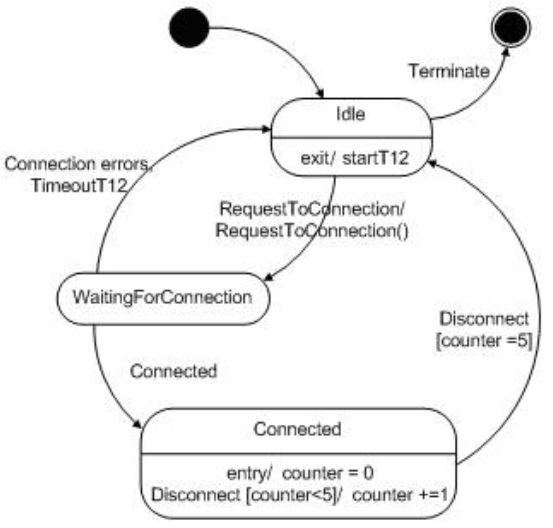
\includegraphics[width=0.5\textwidth]{stateTransitionExample.png}
\end{center}

Прямоугольниками со скруглёнными углами рисуются состояния, у состояния есть имя и (опционально) действия, выполняемые в состоянии (например, действие по выходу или внутренний переход по событию, как у Connected --- получив событие Disconnect, оно проверяет счётчик, и если счётчик меньше 5, он увеличивается на 1 и мы остаёмся в том же состоянии). Состояния связаны переходами, над переходом пишется событие, которое инициирует переход и, опционально, стражник (guard) (логическое условие, которое должно быть истинно, чтобы переход состоялся) и действие, выполняемое при переходе. События со стражниками должны быт взаимно исключающими, недетерминированные автоматы считаются некорректными. Есть псевдосостояния начала и конца, переход из псевдосостояния начала происходит мгновенно, переход в состояние конца заканчиввает исполнение.

Внешне диаграммы конечных автоматов похожи на диаграммы активностей, но есть важные семантические различия:

\begin{itemize}
	\item На диаграмме активностей рисуются активности, система в них не задерживается, а сразу переходит дальше; на диаграмме конечных автоматов рисуются состояния --- стабильные отрезки жизненного цикла объекта, в которых он находится большую часть времени и может из них выйти только если что-то произойдёт;
	\item Полезная работа на диаграммах активностей производится в активностях, на диаграммах автоматов --- как правило, при переходе;
	\item Диаграммы активностей моделируют один метод объекта (или какую-то функцию или что-то такое), диаграммы конечных автоматов --- целый объект (состояния моделируются полями объекта).
\end{itemize}

Более подробно про синтаксис:

\begin{center}
	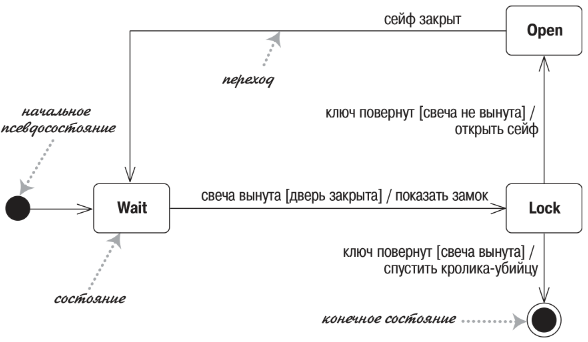
\includegraphics[width=\textwidth]{stateTransitionSyntax.png}
	\attribution{М. Фаулер, UML. Основы}
\end{center}

Внутри состояния могут быть:

\begin{itemize}
	\item entry activity --- то, что делается при входе в состояния по любому из переходов;
	\item exit activity --- то, что делается при выходе из состояния по любому исходящему переходу (и входная, и выходная деятельность --- это, как правило, вызовы метода);
	\item do activity --- деятельность, выполняющаяся всегда, когда система находится в таком-то состоянии (например, попытки подключения к сети для мобильного телефона);
	\item внутренний переход --- переход по событию, который ведёт в то же состояние и не приводит к срабатыванию entry и exit activity. Переход вполне может быть полноценным переходом в то же состояние (рисуется как петля в графе), тогда entry и exit activity работают как обычно, хоть состояние и не меняется.
\end{itemize}

Событие, кстати, это нечто внешнее по отношению к системе, на что система может реагировать. Примеры событий --- действие пользователя, сетевой пакет, считывание символа (если речь идёт об автоматном лексическом анализаторе, который, кстати, хоть и несколько необычный, но тоже пример реактивной системы, которая прекрасно моделируется конечными автоматами).

Надпись на переходе имеет следующий синтаксис: \verb|[<trigger> [‘,’ <trigger>]* [‘[‘ <guard>’]’] [‘/’ <behavior-expression>]]| --- один переход может реагировать на несколько событий сразу, иметь опционального стражника (в квадратных скобках) и через слеш действие (вызов метода или отсылку к диаграмме активностей, которая поясняет, что нужно делать при переходе).

Вот более содержательный пример автомата из работ Д.В. Кознова. Пример демонстрирует порядок работы мобильного телефона, начиная с включения и ввода PIN-кода и заканчивая подключением к сети:

\begin{center}
	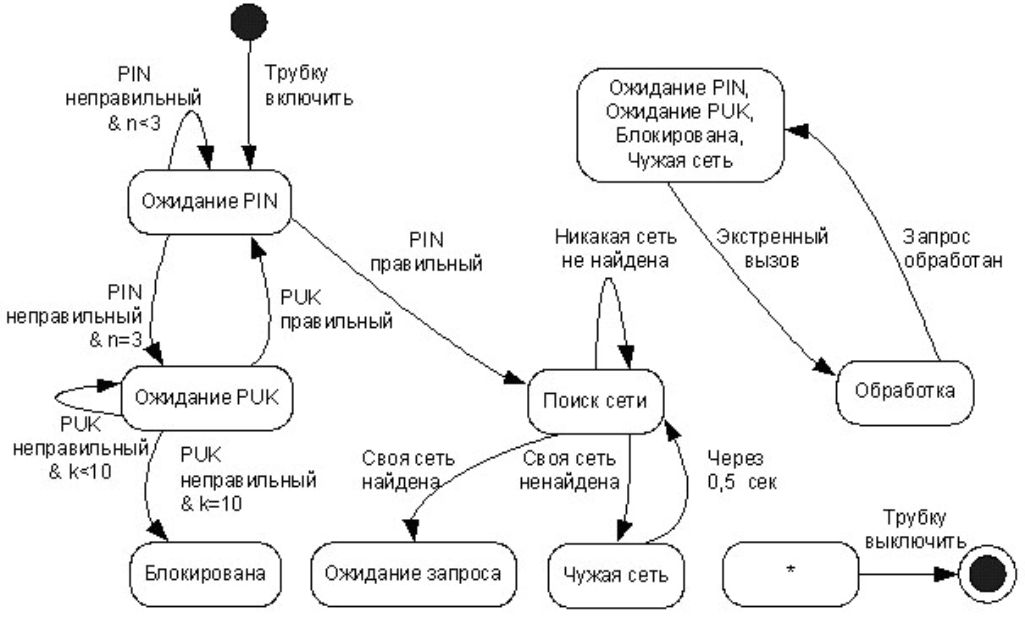
\includegraphics[width=0.7\textwidth]{stateTransitionExample2.png}
\end{center}

Тут используется неканоничный синтаксис с псевдосостоянием ``все состояния'', из которого ведёт переход в конечное псевдосостояние (чтобы не рисовать переход из каждого состояния в конечное) и используются не совсем каноничные надписи над переходами. Связано это с тем, что в те времена, когда на матмехе делались работы по диаграммам конечных автоматов, UML 2 ещё не было, а в UML первых версий синтаксис диаграмм конечных автоматов был менее проработан.

Более продвинутый синтаксис современных диаграмм конечных автоматов позволяет нарисовать пример выше более канонично. Есть вложенные состояния с переходами сразу из всех внутренних состояний:

\begin{center}
	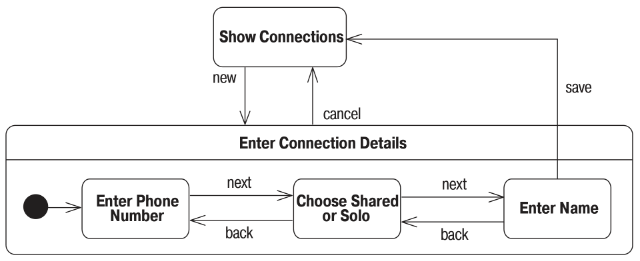
\includegraphics[width=\textwidth]{stateTransitionNestedStates.png}
	\attribution{М. Фаулер, UML. Основы}
\end{center}

Тут состояние <<Enter connection details>> содержит внутри свой конечный автомат, который начинает работать со стартового псевдосостояния когда выполняется переход <<new>>. При этом переход <<save>> возможен только из состояния <<Enter Name>>, а вот переход <<cancel>> возможен из любого вложенного состояния (это замена нестандартному псевдосостоянию со звёздочкой из диаграммы выше).

Ещё бывают параллельные состояния и псевдосостояние истории:

\begin{center}
	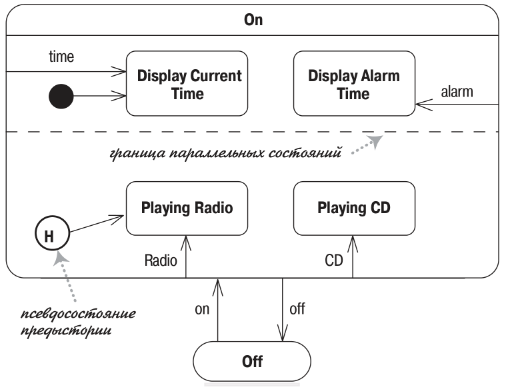
\includegraphics[width=0.7\textwidth]{stateTransitionParallelStates.png}
	\attribution{М. Фаулер, UML. Основы}
\end{center}

Это часы с радио и будильником. Проигрывание звука и время работают независимо, поэтому по сути это два автомата, работающих параллельно (что и показывает горизонтальная прерывистая линия, разделяющая параллельные подавтоматы). Стрелки от объемлющего состояния к вложенным означают, что система, находясь в объемлющем состоянии, реагирует на такие-то события и изменяет внутреннее состояние (например, часы по умолчанию показывают текущее время, но если пользователь нажал на кнопку <<будильник>>, начинает показывать время, на которое будильник установлен). Псевдосостояние истории запоминает последнее вложенное состояние, в котором находился автомат, и возвращает автомат в него. Например, часы по умолчанию включают радио, но если пользователь включил воспроизведение компакт-дисков (если кто помнит, что это такое) и выключил часы, то при следующем включении они снова будут проигрывать компакт-диски.

А вот так рисуются активности внутри состояния:

\begin{center}
	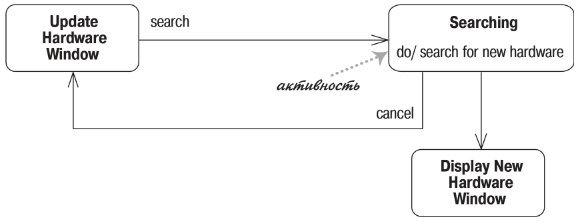
\includegraphics[width=\textwidth]{stateTransitionInternalEventExample.png}
	\attribution{М. Фаулер, UML. Основы}
\end{center}

А вот так --- внутренние переходы и entry/exit-события, о которых шла речь выше:

\begin{center}
	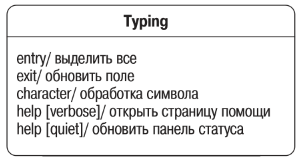
\includegraphics[width=0.5\textwidth]{stateTransitionInternalEvents.png}
	\attribution{М. Фаулер, UML. Основы}
\end{center}

\end{document}
